\chapter{Results and Discussion}
This chapter goes over the results gathered for each method. Accuracy, Loss, SSIM, PSNR and Naturalness study are all used to evaluate each method's performance. Each method is also tested and evaluated on the colourisation of historical photos, and restoration of old coloured photos.
\section{Training results}
After training each model for two weeks, their metrics have been recorded. Below are the results gathered from both AutoEncoders and cGAN.




\subsection{AutoEncoder training results}
Both AutoEncoders were trained for 50 epochs. Accuracy and Loss were recorded during training. The \textbf{accuracy} is calculated by totalling up the number of correctly predicted pixels and dividing it by the total number of pixels in the image. The \textbf{Loss} is another way of measuring similarity, and the goal is to minimise this loss.
Both, training and \textbf{validation loss and accuracy} metrics are shown together. The recorded validation metric is used to determine the model's performance.

\begin{center}
\begin{tabular}{||c c c c||} 
 \hline
  AutoEncoder & Val accuracy & Val loss & Optimal epoch \\ [0.5ex] 
 \hline\hline
 Simple AutoEncoder & 67\% &  0.0095 & 50\\ 
 \hline
 Global AutoEncoder & 69\% & 0.00917 & 45\\
 \hline

\end{tabular}
\end{center}

Table 1. Above shows the training results gathered from two AutoEncoder methods. Out of both models, The Global AutoEncoder has performed the best in terms of accuracy (near 70\%) and low loss (0.0091). This suggests that having a global feature extractor can lead to improvements in colourisation.


\subsubsection*{Simple AutoEncoder Loss/Accuracy graph}
\addcontentsline{toc}{subsubsection}{Simple AutoEncoder Loss/Accuracy graph}
\begin{figure}[H]
    \centering
    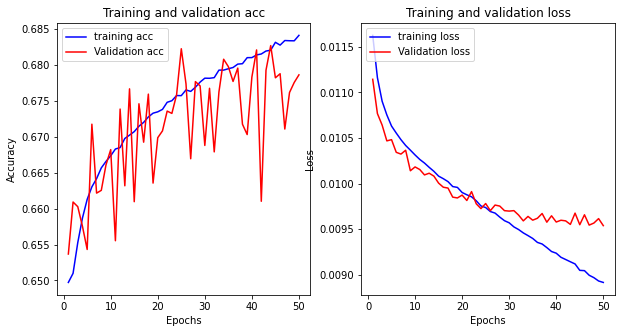
\includegraphics[width=0.7\columnwidth]{sections/figures/autoencoder1_history_loss.png}
    \caption{Simple AutoEncoder training history over 50 epochs}
    \label{fig:my_label}
\end{figure}

In Figure 4.1, you can see the training progress of the Simple Autoencoder. The model was trained for 50 epochs, which took 24 hours to complete. The left graph demonstrates the \textbf{accuracy} for both validation and training sets, while the right graph displays the \textbf{loss} values for both sets. Notice how the validation accuracy has a decent ascending trend, although there is some fluctuation. This is likely due to having a small batch size of 32. The best validation accuracy was \textbf{67\%, achieved at epoch 50}. Whereas the validation loss decreases between 0 and 20 epochs, then levels off and eventually reaches a good \textbf{validation loss of 0.0095} at epoch 50.

\subsubsection*{Global AutoEncoder Loss/Accuracy graph}
\addcontentsline{toc}{subsubsection}{Global AutoEncoder Loss/Accuracy graph}
\begin{figure}[H]
    \centering
    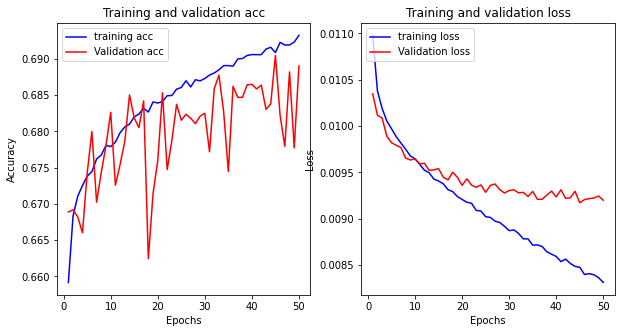
\includegraphics[width=0.7\columnwidth]{sections/figures/autoencoder2_history_loss.png}
    \caption{Global AutoEncoder training history for 50 epochs}
    \label{fig:my_label}
\end{figure}
Here, in Figure 4.2, you can see the recorded history of the Global AutoEncoder training progress. The model has been trained for 50 epochs. However, this method took more time to complete training (2 days) due to it having more parameters to tune. The left graph depicts an upward trend in validation accuracy, though fluctuations continue to be an issue. Whereas in the right graph you can see a similar pattern to the last AutoEncoder, but it drops more quickly and levels out at an early epoch of 10. The \textbf{best validation accuracy was 69\% and loss was 0.0091, which was achieved in epoch 45}.
\subsection{cGan training results}


\begin{center}
\begin{tabular}{||c c c||} 
 \hline
  cGan & Discriminator loss & Generator loss \\ [0.5ex] 
 \hline\hline
 Pix2Pix & 0.0001 & 16.880\\ 
 \hline
 ChromaGAN & -0.0013 & 0.0002\\
 \hline

\end{tabular}
\end{center}
Table 2. The above shows the results gathered for both cGAN methods (Pix2Pix and ChromaGAN). Unfortunately, it is difficult to compare both cGAN models since both rely on entirely different loss metrics as Pix2Pix uses \(L1\) loss whereas ChromaGAN relies on Wasserstein loss for both their generator and discriminator. 

\subsubsection*{Pix2Pix Loss graph}
\addcontentsline{toc}{subsubsection}{Pix2Pix Loss graph}
\begin{figure}[H]
    \centering
    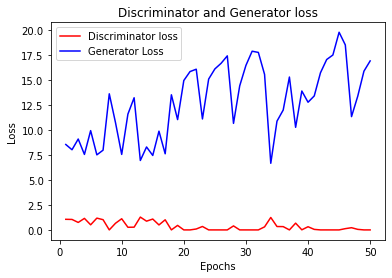
\includegraphics[width=0.7\columnwidth]{sections/figures/pix2pix_history.png}
    \caption{Pix2Pix training history over 50 epochs}
    \label{fig:my_label}
\end{figure}
In figure 4.3, the recorded history of the Pix2Pix cGAN training is shown. The cGAN was trained for 50 epochs, which took 4 days to train using Slurm facility. As observed from the graph, generator and discriminator loss have been plotted. It appears as though the generator is failing to achieve its objective against the discriminator. Despite the generator's loss having an increasing trend, at some points, it has achieved a lower loss, for example in epoch 34. If the model were to be trained for more epochs, the generator would eventually start to win against the discriminator. However, this would take more time for training. Fortunately, I have also trained this model on a smaller dataset (7,000 images) over 400 epochs (refer to Appendix B).

\begin{figure}[H]
    \centering
    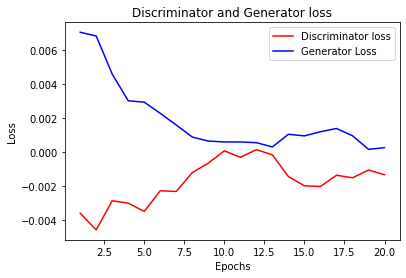
\includegraphics[width=0.7\columnwidth]{sections/figures/chromagan_history.png}
    \caption{ChromaGAN training history for 50 epochs}
    \label{fig:my_label}
\end{figure}
\subsubsection*{ChromaGAN Loss graph}
\addcontentsline{toc}{subsubsection}{ChromaGAN Loss graph}
Figure 4.4 shows the training history for ChromaGAN cGAN. Unlike previous methods, ChromaGAN was only trained for 20 epochs, due to the long training time of 5 days. The generator loss shows a descending trend between the first 8 epochs, then begins to plateau until it ascends slightly between epochs 15 and 17, and then begins to dip again. The discriminator loss mirrors the generator loss. Compared with Pix2Pix, ChromaGAN shows good progress and does not inherit any of the issues seen in the Pix2Pix training history graph, such as the increasing, fluctuating generator loss.








\section{Image colourisation showcase}
\begin{figure}[H]
    \centering
    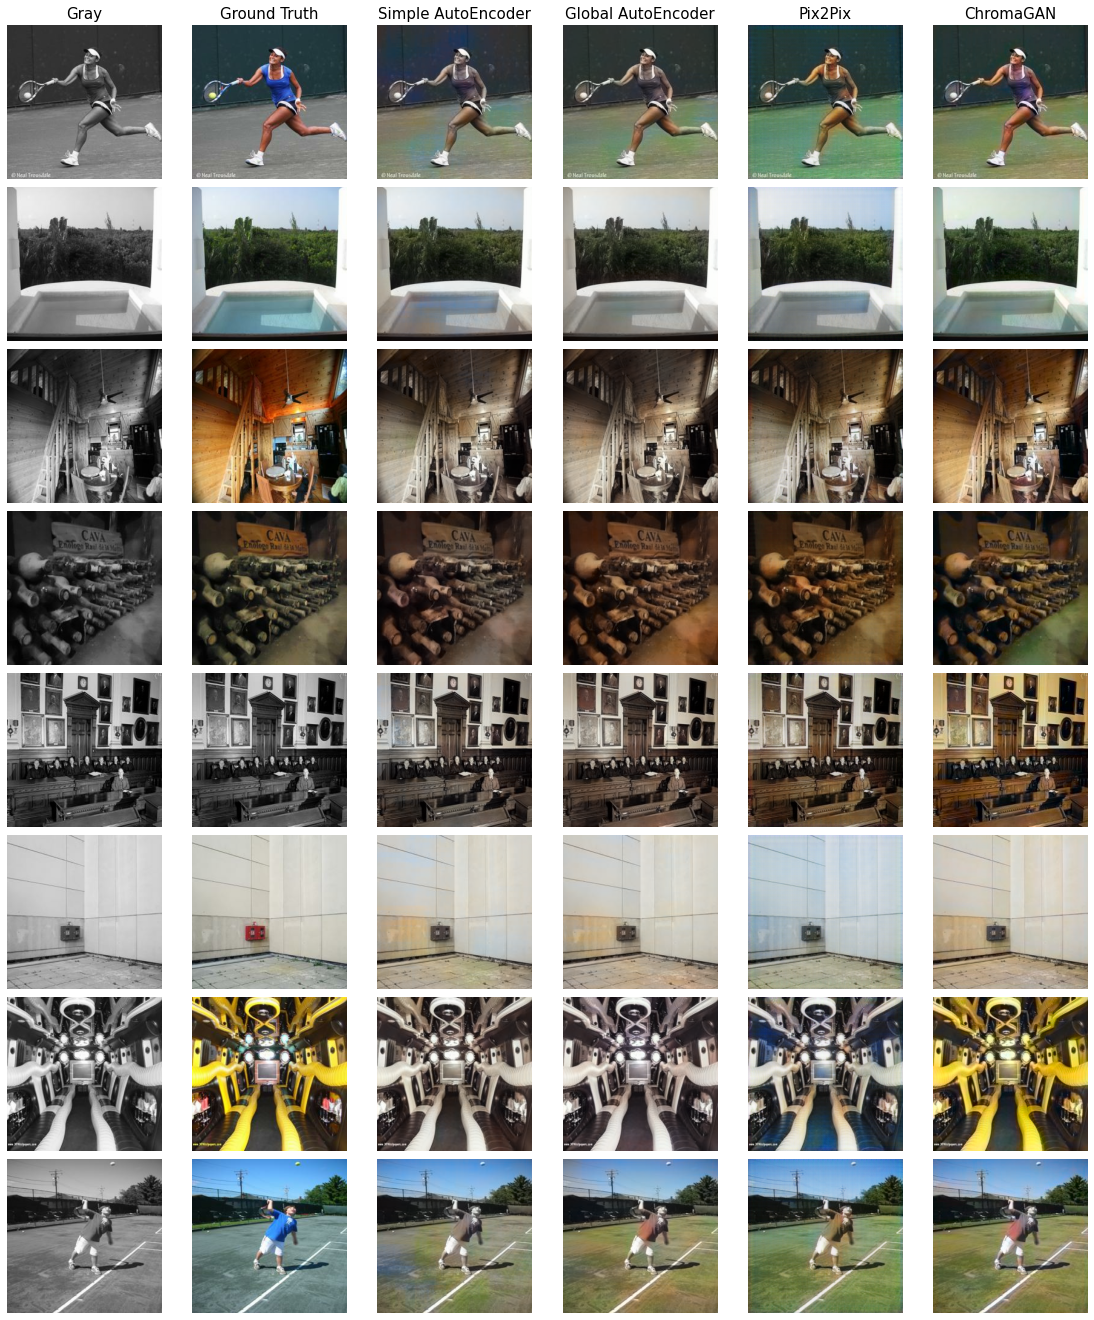
\includegraphics[width=1\columnwidth]{sections/figures/colourisation.png}
    \caption{Eight random images from the test set are colourised. Each row represents an image. The left most column is the grayscale whereas the one next to it is the ground truth. The following three other columns are the three methods used for colourisation.}
    \label{fig:my_label}
\end{figure}


\begin{figure}[H]
    \centering
    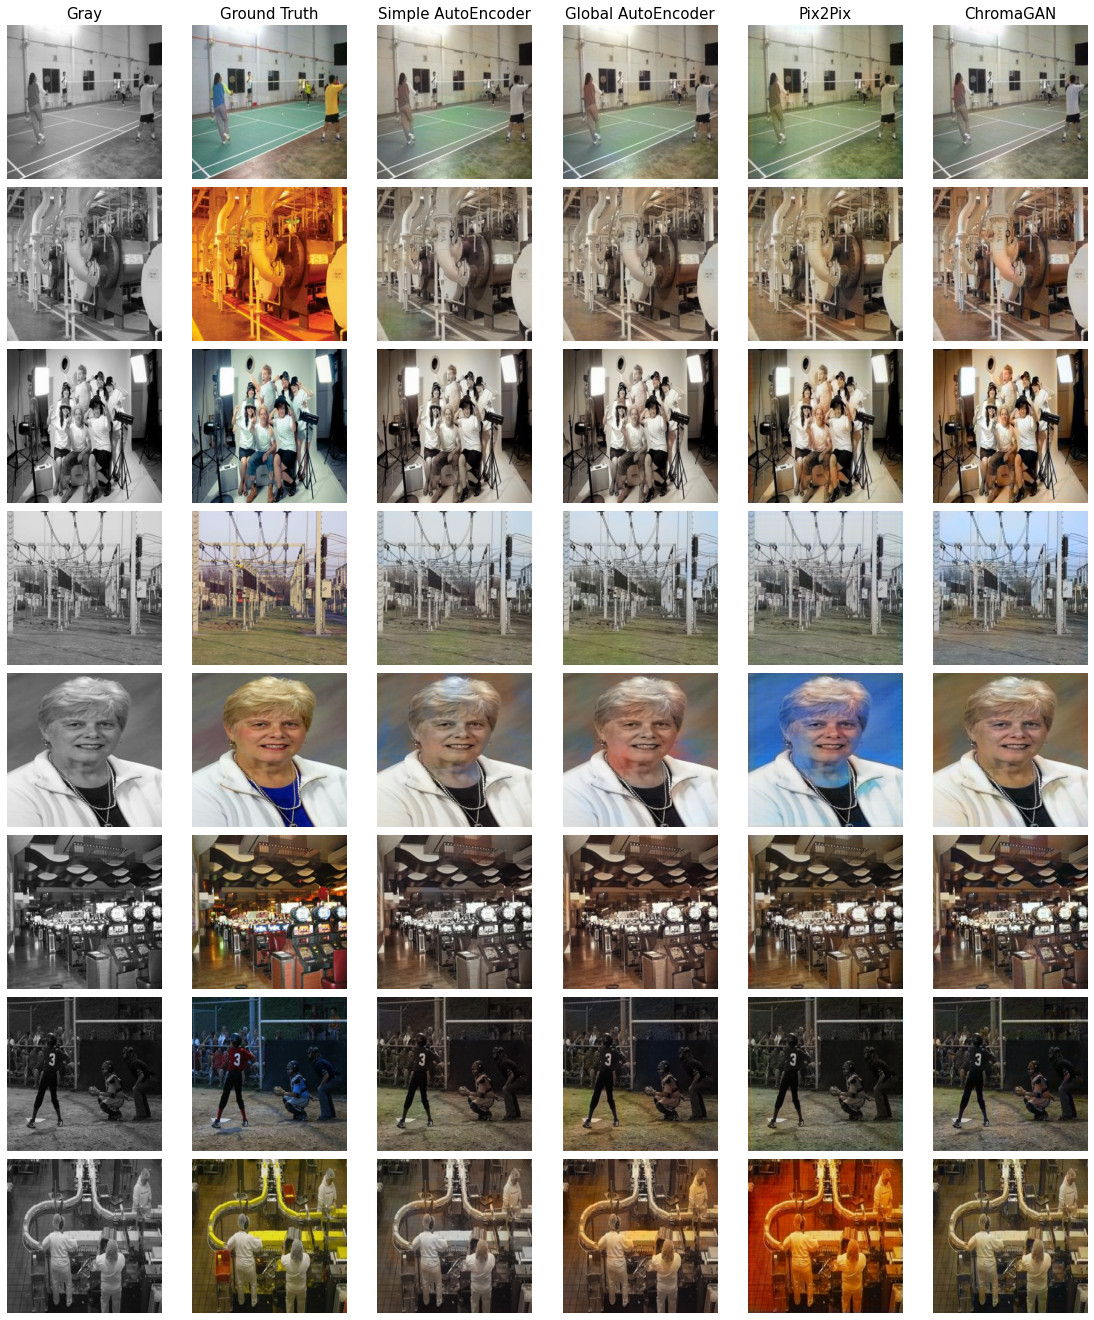
\includegraphics[width=1\columnwidth]{sections/figures/colourisation3.png}
    \caption{Further eight more random images are colourised to showcase each method's colourisation ability.}
    \label{fig:my_label}
\end{figure}



\section{Evaluation}
It was noted in the training results section that accuracy and loss are not reliable metrics to compare between methods since both AutoEncoder and cGAN methods rely on entirely different metrics for evaluation. For this reason, this section will explore evaluation metrics such as \textbf{PSNR}, \textbf{SSIM} and \textbf{natrualness study} which will assist the performance comparison between the methods. 
\subsection{Metric evaluation}
\subsubsection*{Objective score evaluation}
\begin{center}
\begin{tabular}{||c c c||} 
 \hline
  Method & PSNR (dB) & SSIM\\
 \hline
 Simple AutoEncoder & 24.36 & 0.933\\ 
 \hline
 \textbf{Global AutoEncoder} & \textbf{24.45} & \textbf{0.936}\\
 \hline
 Pix2Pix & 23.355 & 0.906\\
 \hline
 ChromaGAN & 23.94 & 0.921\\
 \hline
\end{tabular}
\end{center}
The PSNR and SSIM objective metrics were used to evaluate all mentioned architectures using a test set of 21,000 images.  Here, you can see a correlation between both metrics. For example, the Global AutoEncoder achieves the best PSNR and SSIM score of 24.45 and 0.936 respectively. Whereas, Pix2Pix comes in last, scoring the lowest in PSNR and SSIM scores. Notice how the AutoEncoder class outperforms the cGAN, this may be due to the nature of the AutoEncoder training, which involves iteratively attempts to make the predictions similar and more inclined to the targets, and both, PSNR and SSIM rely on \textbf{similarity}. Whereas the cGAN were trained to make the resulting predictions \textbf{realistic}, which disregards the aim of making it similar, hence why the cGAN performed worse off.


% I evaluated the average PSNR score per method using the test of 21,000 images. PSNR is a metric used to calculate the peak signal-to-noise ratio in decibels between two images. The goal is to maximise the PSNR score. The global AutoEncoder seems to have performed the best and the Simple AutoEncoder closely follows up. ChromaGAN is the third-best model, achieving nearly 24 in average PSNR, whereas Pix2Pix comes last as it scored the lowest. The AutoEncoder class outperforms the cGAN, this may be due to the nature of the AutoEncoder training, which involves iteratively attempts to make the predictions \textbf{similar} and more inclined to the targets, and PSNR score measures the similarity. Whereas the cGAN were trained to make the resulting predictions \textbf{realistic}, which disregards the aim of making it similar, hence why the cGAN performed worse off.


\subsubsection*{Naturalness study evaluation}
\begin{center}
\begin{tabular}{||c c||} 
 \hline
  Method & Naturalness\\
 \hline
 Real Images & 93\%\\ 
 \hline
 Simple AutoEncoder & 45\%\\ 
 \hline
 Global AutoEncoder & 51\%\\
 \hline
 Pix2Pix & 53\%\\
 \hline
 \textbf{ChromaGAN} & \textbf{74}\%\\
 \hline
\end{tabular}
\end{center}
26 participants took part in the naturalness study. The study included real images to provide baseline accuracy. The best performing model was ChromaGAN, which achieved 74\% accuracy. Pix2Pix followed with 53\% accuracy. Global AutoEncoder came in third with 51\%. Simple AutoEncoder had the lowest score of 45\%. None of the methods, however, were able to come close to the real image score of 93\%. This may be due to errors that easily gave away the naturalness of the image. For example, \textbf{visual abstracts} which were seen in the first three methods, also, photos containing humans were turned into zombies as parts of their body remained grey. This was seen throughout the first three models. ChromaGAN managed to perform reasonably well, but the reason it isn't on the same level as real images is likely due to the bland colour palette, which is seen throughout all methods. In contrast to the objective scores, cGAN outperformed the AutoEncoders in this study. This was discussed earlier that the cGAN mainly aims to perform \textbf{realistic} colourisation, which is what this study relies on.



\begin{figure}[H]
    \centering
    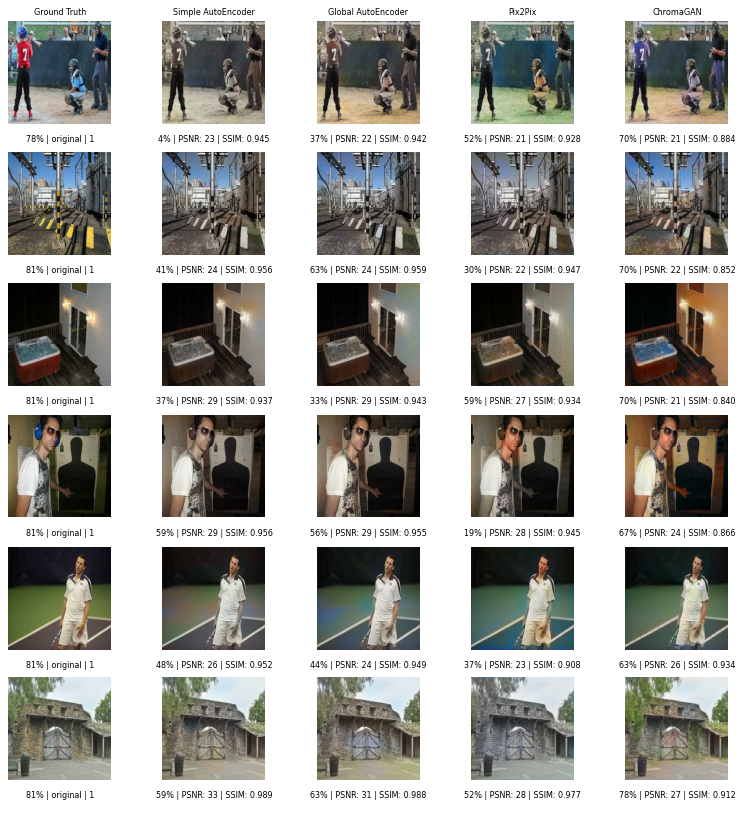
\includegraphics[width=1\columnwidth]{sections/figures/coloured_results.png}
    \caption{For each recoloured image per method, I have added a percentage of users who answered "real" or "fake".}
    \label{fig:my_label}
\end{figure}
Here in Figure 4.5, I've randomly handpicked several images used throughout the naturalness perception study. The left-most column represents the \textbf{ground truth} where the following right columns represent the four methods I have discussed so far. Here, the naturalness percentage score alongside their respective PSNR & SSIM scores.

The first thing I noticed was how the results help depict the behaviour of the observers. For example, some images contain visual abstracts which makes it obvious for the observers to make this "unnatural". Also, some results seem to show little change in percentage even though the contrast or luminosity is slightly tweaked. This shows that the observers are tolerant of minor changes. 

Additionally, you can notice how the cGAN models (pix2pix \& chromaGAN) have performed on average the best in terms of naturalness scores, whereas the two AutoEncoders have scored better in terms of PSNR & SSIM. As discussed in the last section, there does seem to be a clear trade-off between the objective metrics and Naturalness scores. It's fair to assume that the cGAN is likely to be the preferred method even if it has a worse average PSNR & SSIM score. \textbf{In my opinion the scores observed from the human eye (naturalness study) matter more than the scores computed by the computer (PSNR & SSIM)}. Out of all methods, it's observed that the ChromaGAN is the best-suited model for image colourisation. 





\pagebreak
\subsection{Historical photos analysis}
\begin{figure}[H]
    \centering
    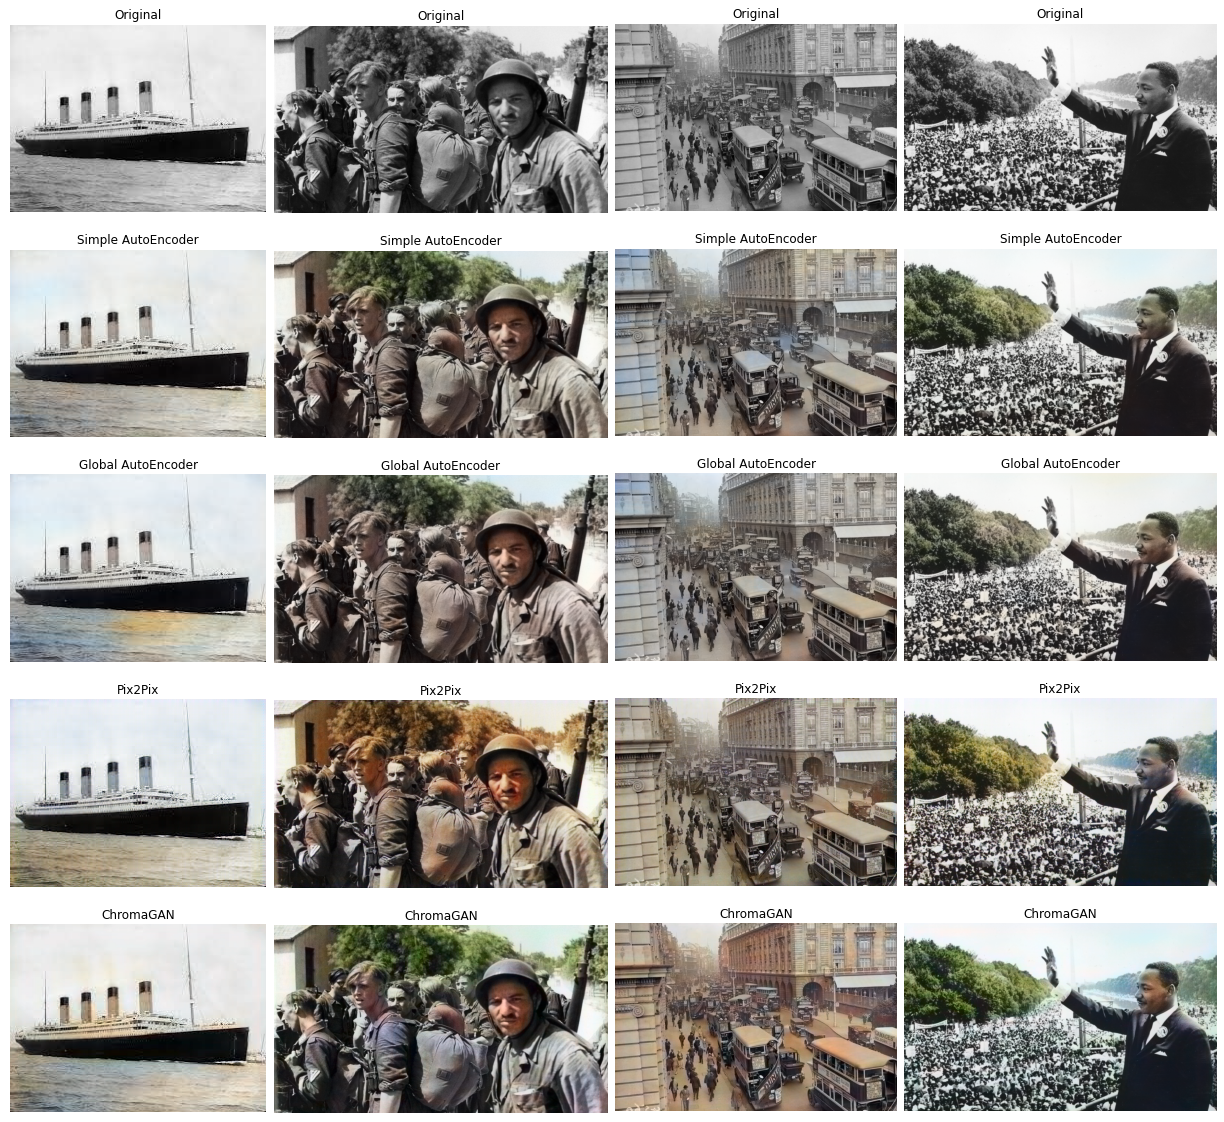
\includegraphics[width=1\columnwidth]{sections/figures/historical_colourised_photos.png}
    \caption{A few historical photos have been picked. Titanic (1912),  French Algerian soldier Gaurding captured German soldiers (1944) and London (1920s), Martin Luther King giving a speech (1963).}
    \label{fig:my_label}
\end{figure}
I've tested each model on historical photos. Figure 4.8 shows the colourisation results. Since there are no ground truths to identify how accurate each model is, it is down to personal judgement. ChromaGAN seems to show the best overall colourisation results as it does a better job colourising people and their surroundings. 

\subsection{Colour restoration analysis}

\begin{figure}[H]
    \centering
    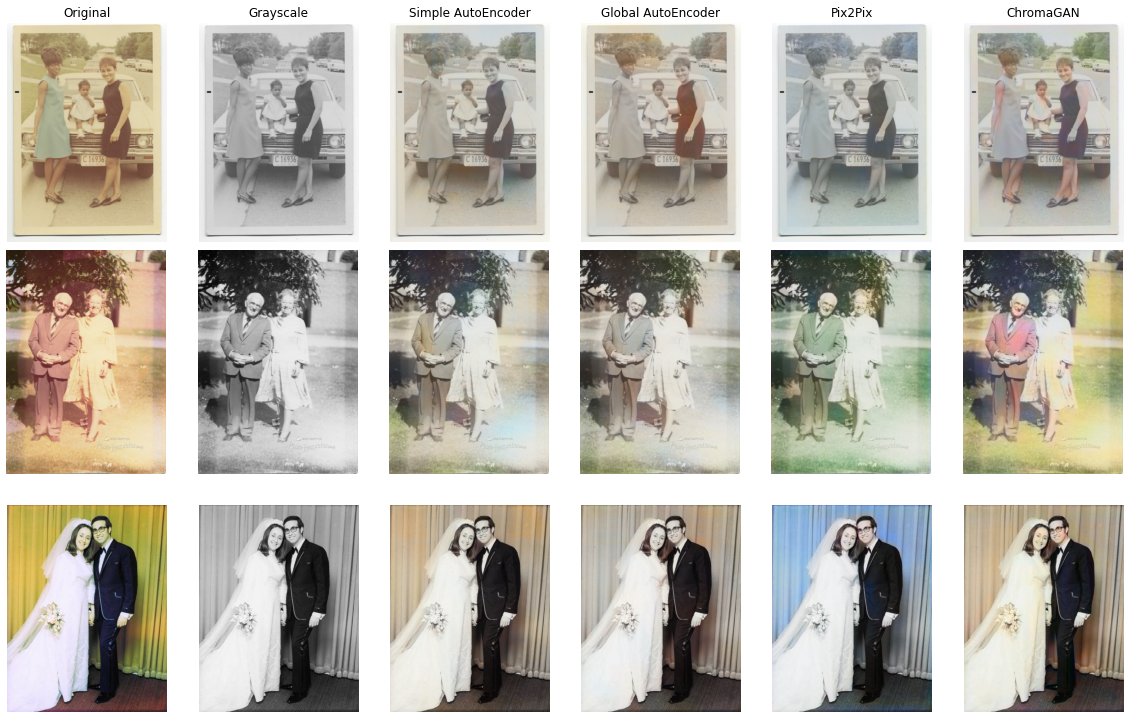
\includegraphics[width=1\columnwidth]{sections/figures/colour_resortation.png}
    \caption{Restoring the colours of a few photos whose colours have faded}
    \label{fig:my_label}
\end{figure}


 I've handpicked three photos that have suffered deterioration in quality due to environmental factors such as poor handling, poor material or ageing. The photos were used to test each model's capabilities for the purpose of restoring colours. 

 Out of all methods, the ChromaGAN model has done a decent job in bringing back the vibrant colours which lacked in the original photos. It even removed the orange hue seen within the first two original images.

 However, not all methods are accurate, for example in the third row, Pix2Pix coloured the curtains blue instead of yellow. 

 It is also important to note that the models cannot remove the fade effect or any other visual abstracts seen in the original image as none of the models were trained to deal with this type of issue, hence why its presence still exists in the resulting images. 
\pagebreak
\section{limitations}
\begin{figure}[H]
    \centering
    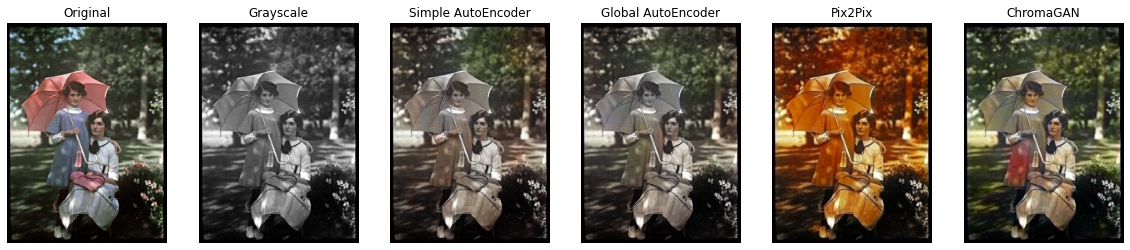
\includegraphics[width=1\columnwidth]{sections/figures/limitation1.png}
    \caption{Limitation example 1}
    \label{fig:my_label}
\end{figure}
Here, it is important to outline a few key limitations observed from all methods. For example, figure 4.10 demonstrates some form of the limitations suffered by each model:

\begin{enumerate}
  \item All methods were trained to colourise images of size 256x256 (except ChromaGAN - 242x242), this means that test images require resizing. Resizing causes distortion which can negatively impact the colourisation process. This is seen in the first three methods.
  \item The colourisation process is biased and will not apply accurate colours to everything. For instance, it failed to colourise the umbrella or the handbag pink. This is because the algorithms were only trained on what they had seen and likely never trained on images consisting of pink umbrellas and pink handbags. 
  \item The predicted colours are also bland, especially complex small objects. This again relates to the last point of bias: The algorithm has a lot to learn before it can learn to colourise more entities using accurate colours.
  \item Incorrect colour placement and visual abstracts are very apparent and seen throughout all models. For instance, the colourisation of Pix2Pix is completely all orange, whereas ChromaGAN has produced a slight reddish visual abstract which can be seen on the dress of the left person. 

\end{enumerate}
Despite mentioning all these limitations, some of the methods such as ChromaGAN manage to do a decent enough job to make the colourisation look convincing, however, still suffer from the limitations mentioned above.




\begin{figure}[H]
    \centering
    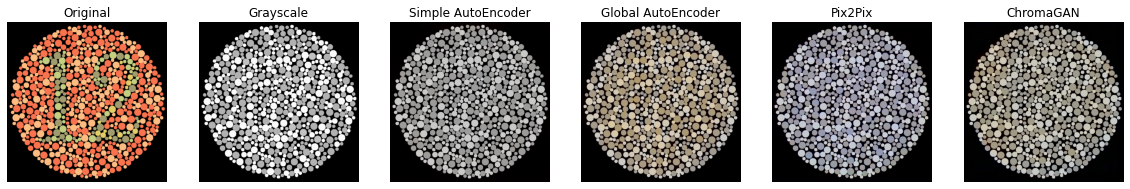
\includegraphics[width=1\columnwidth]{sections/figures/limitation2.png}
    \caption{Limitation example 2}
    \label{fig:my_label}
\end{figure}
Furthermore, the methods are not suitable for colourising synthetic images as demonstrated in figure 4.11. For instance, the colour blind test contains a "12" which is coloured in green. However, as you can observe, the grayscale image completely loses all the information of all the synthetic colours, and if we, the viewers can not see a "12" from a grayscale image then neither can the models. 

\pagebreak
\section{Discussion}
Let's revisit the aims established at the beginning of this investigation:

\begin{enumerate}
  \item Determine the best image colourisation method by carrying out an analysis of deep learning architectures such as AutoEncoders and Conditional Adversarial Networks using quantitative measures such as human assessment and objective metrics.
  \item Investigate whether the objective measures correlate with
human assessment results and determine which measures matter more for the purpose of image colourisation.
\end{enumerate}

Now I believe the first aim has been addressed since judging from the results discussed earlier, I've successfully carried out an analysis of AutoEncoders and cGAN using objective measures (PSNR & SSIM) and human measures (natural perception test). Here, judging from the results, it appears that the cGAN methods provide more realistic results, offering diverse colourisation than AutoEncoders, while AutoEncoders generate results that better match the targets but with colours often seen as less realistic. Here, it was revealed that the human assessment tends to rely more on realistic colourisation, whilst the objective measures relied more on similarity. And it was seen that the cGAN performed better on realism, whereas AutoEncoders were better are similarity.

So there's a clear trade-off between realism and similarity, which raises the second aim established earlier. It's clear that the objective measures do not correlate with human opinion, and this may be because the objective measures only focus on the structural and noise differences, not the colour, which the human volunteers focused on, which makes the objective metrics unreliable in conducting an evaluation for image colourisation. Unfortunately, there does not seem to be any alternative metrics, hence using human-driven study was needed.   

Also, according to this study, ChromaGAN performed consistently the best as it managed to achieve the highest average naturalness study score (73\%) and a reasonably good average PSNR/SSIM score, making ChromaGAN the best-suited algorithm for image colourisation.




